\documentclass[a4paper, 12pt]{article}

\usepackage{listings}
\usepackage{indentfirst}
\usepackage{graphicx}
\usepackage{pdfpages}

\usepackage{color}

\definecolor{mygreen}{rgb}{0,0.6,0}
\definecolor{mygray}{rgb}{0.5,0.5,0.5}
\definecolor{mymauve}{rgb}{0.58,0,0.82}

\lstset{ 
  backgroundcolor=\color{white},   % choose the background color; you must add \usepackage{color} or \usepackage{xcolor}; should come as last argument
  basicstyle=\footnotesize,        % the size of the fonts that are used for the code
  breakatwhitespace=false,         % sets if automatic breaks should only happen at whitespace
  breaklines=true,                 % sets automatic line breaking
  captionpos=b,                    % sets the caption-position to bottom
  commentstyle=\color{mygreen},    % comment style
  deletekeywords={...},            % if you want to delete keywords from the given language
  escapeinside={\%*}{*)},          % if you want to add LaTeX within your code
  extendedchars=true,              % lets you use non-ASCII characters; for 8-bits encodings only, does not work with UTF-8
  keepspaces=true,                 % keeps spaces in text, useful for keeping indentation of code (possibly needs columns=flexible)
  keywordstyle=\color{blue},       % keyword style
  language=Octave,                 % the language of the code
  morekeywords={*,...},            % if you want to add more keywords to the set
  numbers=left,                    % where to put the line-numbers; possible values are (none, left, right)
  numbersep=5pt,                   % how far the line-numbers are from the code
  numberstyle=\tiny\color{mygray}, % the style that is used for the line-numbers
  rulecolor=\color{black},         % if not set, the frame-color may be changed on line-breaks within not-black text (e.g. comments (green here))
  showspaces=false,                % show spaces everywhere adding particular underscores; it overrides 'showstringspaces'
  showstringspaces=false,          % underline spaces within strings only
  showtabs=false,                  % show tabs within strings adding particular underscores
  stepnumber=2,                    % the step between two line-numbers. If it's 1, each line will be numbered
  stringstyle=\color{mymauve},     % string literal style
  tabsize=2,	                   % sets default tabsize to 2 spaces
  title=\lstname                   % show the filename of files included with \lstinputlisting; also try caption instead of title
}

%===========================================%
%=               Credits                   =%

\author{Name}
\title{Title}

%=                                         =%
%===========================================%

%===========================================%
%=               BEGIN                     =%

\begin{document}
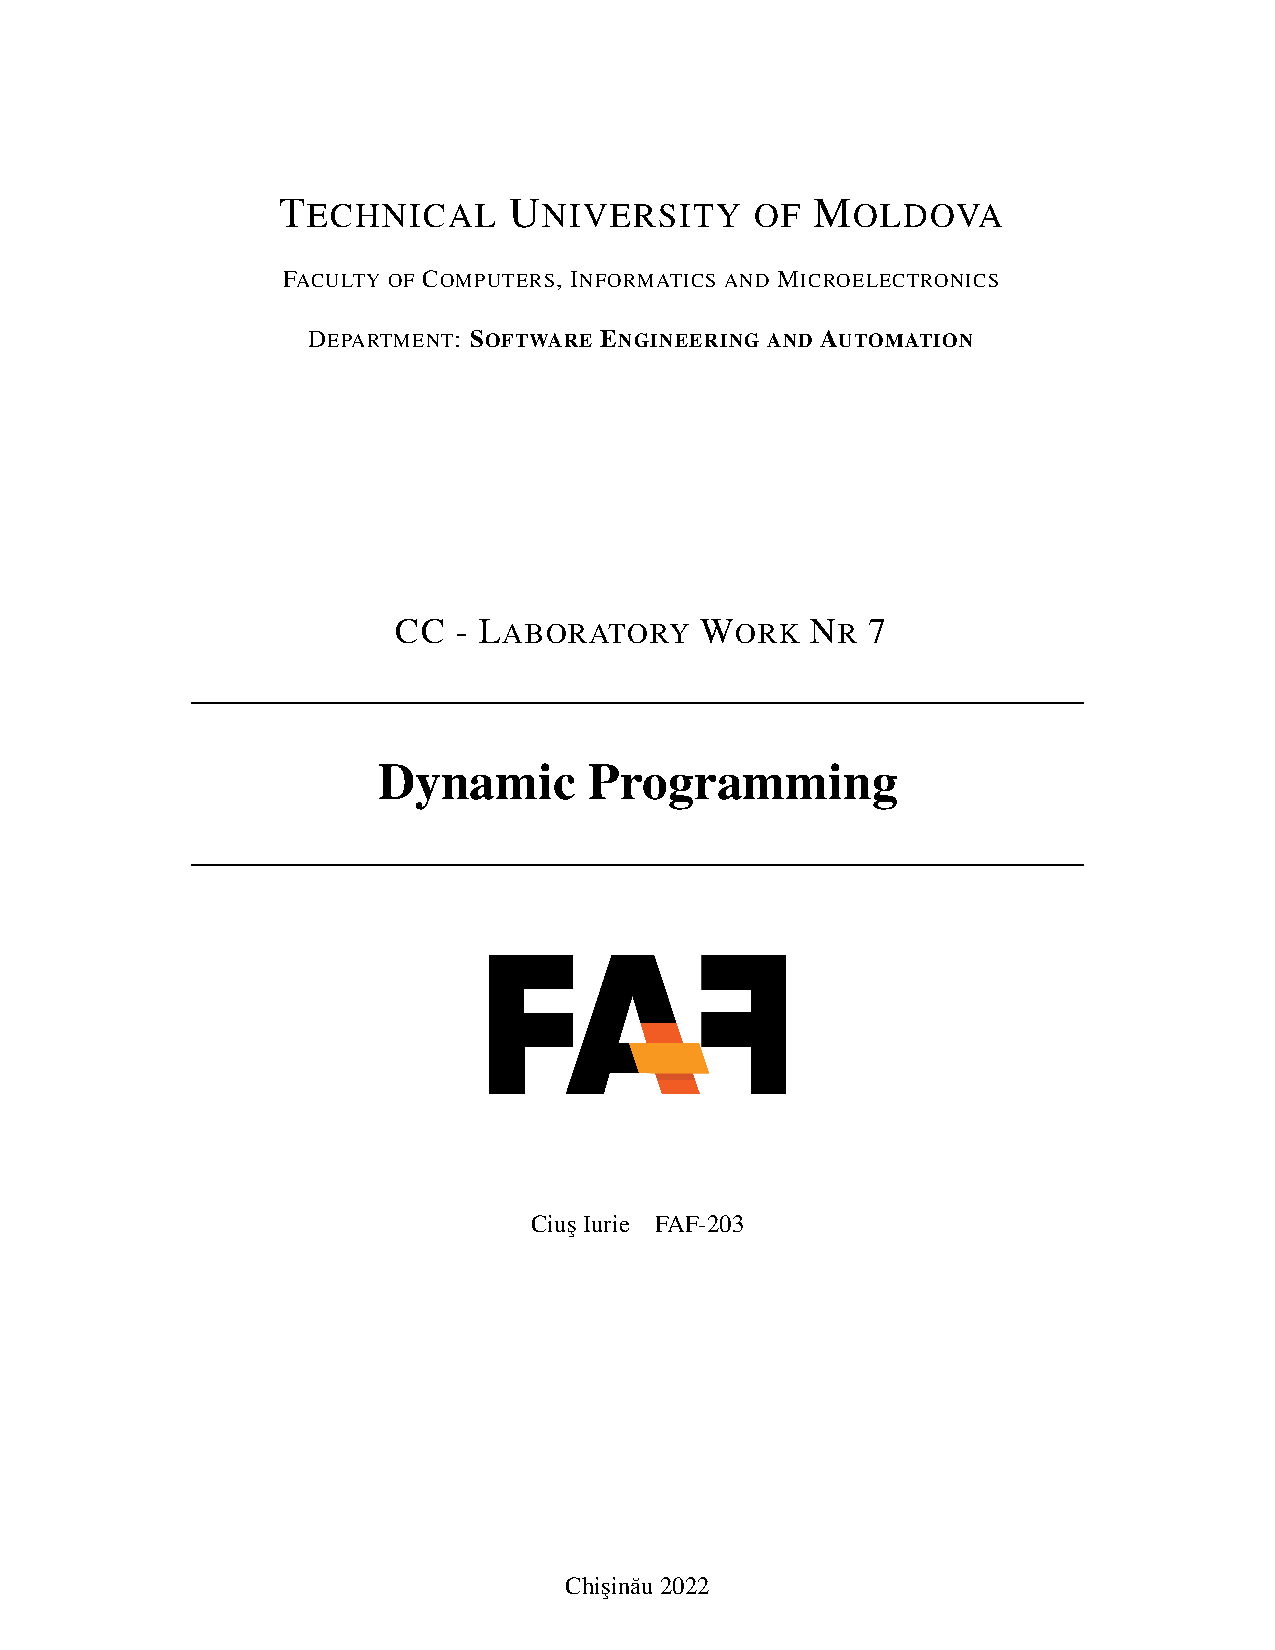
\includepdf[pages={1}]{title.pdf}
\tableofcontents
\newpage

\section{Algorithm Analysis}

Algorithm analysis is an important part of computational complexity theory, which provides
theoretical estimation for the required resources of an algorithm to solve a specific computational problem. Analysis of algorithms is the determination of the amount of time and space
resources required to execute it.

\subsection{Introduction}

Dynamic Programming (DP) is an algorithmic technique for solving an
optimization problem by breaking it down into simpler subproblems
and utilizing the fact that the optimal solution to the overall problem
depends upon the optimal solution to its subproblems.

Let’s take the example of the Fibonacci numbers. As we all know,
Fibonacci numbers are a series of numbers in which each number is
the sum of the two preceding numbers. The first few
Fibonacci numbers are 0, 1, 1, 2, 3, 5, and 8, and they continue on from there.

If we are asked to calculate the nth Fibonacci number, we can do that with the following equation,

$$
      Fib(n) = Fib(n-1) + Fib(n-2), for n > 1
$$

As we can clearly see here, to solve the overall problem (i.e. Fib(n)), we broke it down into two smaller subproblems (which are Fib(n-1) and Fib(n-2)). This shows that we can use DP to solve this problem.


\subsection{Control questions:}

\begin{itemize}
      \item Describe the dynamic programming method.
      \item Why is this method called dynamic programming?
      \item What is the difference between the divide et impera method and the dynamic programming?
      \item What is the classification of dynamic programming problems?
      \item What happens in the case when the costs of graph arcs processed with dijkstra and floyd algorithms are negative?
\end{itemize}

\subsection{Theoretical Notes}

A problem solvable by dynamic programming method it must first be brought to a discreet form in time. Decisions to be taken take to get a result must be able to take it step by step. Of also very important is the order in which they are taken. Dynamic programming is (and you don't take these rows as a definition) essentially a decision-making process in several stages: in the initial state of the problem we make the first decision, which determines a the new state of the problem in which we make a decision. The dynamic term is relates to this very thing: the problem is solved in stages time-dependent. Variables, or functions that describe each the stage must be so defined as to completely describe a process, so for this we will have to answer two questions:

\begin{itemize}
      \item what is the initial stage (in which case we are dealing with a top-down decision-making) or what is the final stage (in which case we are dealing with an upward decision-making process)?
      \item what is the rule by which we go from one stage to another? Of usually this rule is expressed by a recurrence.
\end{itemize}

Because, we are dealing with a problem that is solved in May many stages, all we have to do is see how we make the decisions from one stage to another.

For example, the problem of calculating Fibonaci numbers is falls into the category of dynamic programming because:

\begin{itemize}
      \item it is a phased process;
      \item each step k corresponds to the calculation of the k-th number Fibonacci;
      \item there is only one decision to move to a higher stage;
\end{itemize}

In the following, by strategy we mean a series of decisions. According to Bellman's principle, called the principle of optimality we have:

\textbf{A strategy has the property that whatever its original state and the initial decision, the remaining decisions must constitute an optimal strategy regarding the state of the previous decision.}

\subsection{Description of The Algorithms}

\subsubsection*{Dijkstra’s shortest path algorithm}

\begin{enumerate}
      \item Create a set sptSet (shortest path tree set) that keeps track of vertices included in the shortest-path tree, i.e., whose minimum distance from the source is calculated and finalized. Initially, this set is empty.
      \item  Assign a distance value to all vertices in the input graph. Initialize all distance values as INFINITE. Assign distance value as 0 for the source vertex so that it is picked first.
      \item While sptSet doesn’t include all vertices
            \begin{itemize}
                  \item Pick a vertex u which is not there in sptSet and has a minimum distance value.
                  \item Include u to sptSet.
                  \item Update distance value of all adjacent vertices of u. To update the distance values, iterate through all adjacent vertices. For every adjacent vertex v, if the sum of distance value of u (from source) and weight of edge u-v, is less than the distance value of v, then update the distance value of v.
            \end{itemize}
\end{enumerate}

\subsubsection*{Floyd Warshall Algorithm}

We initialize the solution matrix same as the input graph matrix as a first step. Then we update the solution matrix by considering all vertices as an intermediate vertex. The idea is to one by one pick all vertices and updates all shortest paths which include the picked vertex as an intermediate vertex in the shortest path. When we pick vertex number k as an intermediate vertex, we already have considered vertices {0, 1, 2, .. k-1} as intermediate vertices. For every pair (i, j) of the source and destination vertices respectively, there are two possible cases.

\begin{itemize}
      \item k is not an intermediate vertex in shortest path from i to j. We keep the value of dist[i][j] as it is.
      \item  k is an intermediate vertex in shortest path from i to j. We update the value of dist[i][j] as dist[i][k] + dist[k][j] if dist[i][j] > dist[i][k] + dist[k][j]
\end{itemize}

\section{Code}
\subsection{Implementation}

\subsubsection*{Djikstra Algorithm}
\lstinputlisting[language=Python]{djikstra.py}

\subsubsection*{Floyd Warshall Algorithm}
\lstinputlisting[language=Python]{floyd.py}

\subsection{Complexity of the Algorithms}

\subsubsection*{Djikstra}

Time Complexity of Dijkstra's Algorithm is $O ( V^2 )$ but with min-priority queue it drops down to $O ( V + E l o g V )$ .

\subsubsection*{Floyd Warshall}

The Floyd-Warshall algorithm is a graph-analysis algorithm that calculates shortest paths between all pairs of nodes in a graph. It is a dynamic programming algorithm with $O(|V|^3)$ time complexity and $O(|V|^2)$ space complexity.

\subsection{Graphs}

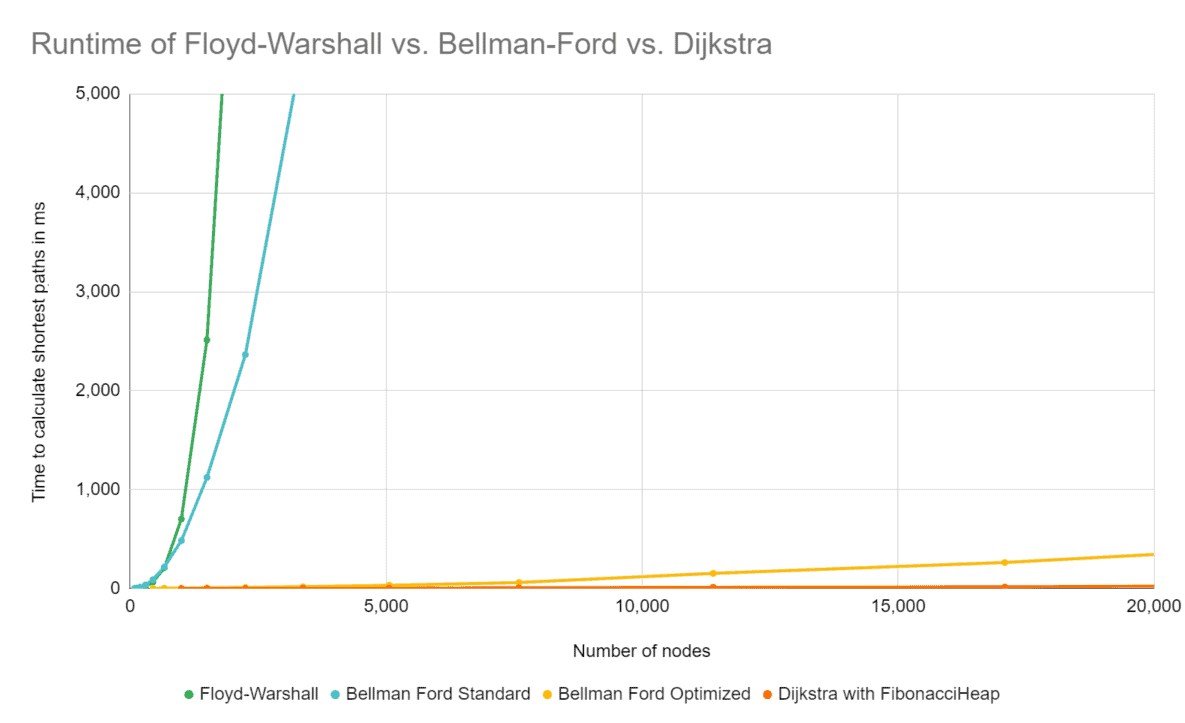
\includegraphics[width=14cm]{img1.png}

\section{Conclusion}

To conclude, the current piece of work represents my personal implementation of 2 algorithms - Djikstra and Floyd. The programming
language I chose is Python. The results show the time performance in mili-seconds
based on the N. As you can see in the Figure 1, the Djikstra algorithms
performed the best with a complexity of O(1), while the second one - $O(2^n)$.

\subsection{References}

\begin{itemize}
      \item https://github.com/IuraCPersonal
\end{itemize}


\end{document}